\newif\ifsolutions
\solutionstrue % Show solutions
%\solutionsfalse % Hide solutions

\documentclass{article}
\usepackage{geometry}
\geometry{margin=1in}
\usepackage{tikz}
\usepackage{amssymb}

% fleqn allows setting indent of display math
\usepackage[fleqn]{amsmath}
\setlength{\mathindent}{0pt} % Set indent
% Disable equation numbering (https://tex.stackexchange.com/a/360378)
\makeatletter
\renewcommand\tagform@[1]{}
\makeatother

% Allow Unicode (some, e.g., © and £ at least)
% https://tex.stackexchange.com/questions/370278/is-there-any-reason-to-use-inputenc
\usepackage[utf8]{inputenc}

% Hyperlinks
\usepackage{hyperref}
\hypersetup{colorlinks=true, urlcolor=blue, linkcolor=blue}

% Prevent indentation of paragraphs
\setlength\parindent{0pt}
\setlength{\parskip}{\baselineskip}

% Spacing above/below equations
% https://tex.stackexchange.com/a/69678
\AtBeginDocument{%
 \abovedisplayskip=-\parskip
 \abovedisplayshortskip=-\parskip
 \belowdisplayskip=0pt
 \belowdisplayshortskip=0pt
}

% Allow 3 additional subsection levels
% https://tex.stackexchange.com/a/60212
\usepackage{titlesec}
\setcounter{secnumdepth}{6}
% H4 in HTML
\titleformat{\paragraph}{\normalfont\normalsize\bfseries}{\theparagraph}{1em}{}
\titlespacing*{\paragraph}{0pt}{3.25ex plus 1ex minus .2ex}{1.5ex plus .2ex}
% H5 in HTML
\titleformat{\subparagraph}{\normalfont\normalsize\bfseries}{\thesubparagraph}{1em}{}
\titlespacing*{\subparagraph}{0pt}{3.25ex plus 1ex minus .2ex}{1.5ex plus .2ex}
% H6 in HTML
\titleformat{\subsubparagraph}{\normalfont\normalsize\bfseries}{\thesubsubparagraph}{1em}{}
\titlespacing*{\subsubparagraph}{0pt}{3.25ex plus 1ex minus .2ex}{1.5ex plus .2ex}

% So enumerate at all levels is numbers
% https://tex.stackexchange.com/questions/78842/nested-enumeration-numbering
\renewcommand{\labelenumii}{\arabic{enumii}.}
\renewcommand{\labelenumiii}{\arabic{enumiii}.}
\renewcommand{\labelenumiv}{\arabic{enumiv}.}

\renewcommand{\mbox}{\text}
\newcommand{\ds}[0]{\displaystyle}
\newcommand{\ihat}[0]{\hat{\boldsymbol{\imath}}}
\newcommand{\jhat}[0]{\hat{\boldsymbol{\jmath}}}
\newcommand{\khat}[0]{\hat{\boldsymbol{k}}}
\newcommand{\xhat}[0]{\hat{\mathbf{x}}}
\newcommand{\yhat}[0]{\hat{\mathbf{y}}}
\newcommand{\zhat}[0]{\hat{\mathbf{z}}}
\newcommand{\rhat}[0]{\hat{\mathbf{r}}}
\newcommand{\bfvec}[1]{\vec{\mathbf{#1}}}
\newcommand{\bfcdot}[0]{\boldsymbol{\cdot}}

\usepackage{fancyhdr}
\pagestyle{fancy}
\lhead{Gauss's Law}
\rhead{\thepage}
\fancyfoot{}

\begin{document}

\section{Introduction}

Gauss's law is derived from Coulomb's law, so they are both equally valid. Coulomb's law can always be used to find the electric field due to a continuous charge distribution when the charge density is known. Gauss's law is only useful for computing the electric field for certain continuous charge distributions. The list includes all of the charge distributions considered in the Enclosed Charge activity:

\begin{itemize}

  \item near the center of a long and uniformly charged line,

  \item near the center of a long and uniformly charged cylindrical shell,

  \item at any location for a uniformly charged spherical shell, and

  \item near the center of a large and uniformly charged sheet.

\end{itemize}

Gauss's law can also be used to find the electric field due to a long and uniformly charged solid cylinder and a uniformly charged solid sphere because they can be created by nesting shells together and using a superposition argument.

Gauss's law states that the total electric flux through any closed surface is proportional to the total charge inside the surface.

$$\text{Gauss's law}\qquad\oint \bfvec{E}\cdot d\mathbf{A}=\frac{Q_{\text{encl}}}{\epsilon_o}$$

In the following diagram, a closed spherical surface is shown. Gauss's law states that if we add all of the differential fluxes $\bfvec{E}\cdot d\mathbf{A}$ over the closed surface, the result will be ${Q_{\text{encl}}}/{\epsilon_o}$. The surface does not need to be spherical -- Gauss's law is valid for any closed surface. Any imaginary surface that we use in Gauss's law is referred to as a Gaussian surface.



% Gradient Info
  
\tikzset {_hjttd0z14/.code = {\pgfsetadditionalshadetransform{ \pgftransformshift{\pgfpoint{89.1 bp } { -108.9 bp }  }  \pgftransformscale{1.32 }  }}}
\pgfdeclareradialshading{_zlfwnqdgv}{\pgfpoint{-72bp}{88bp}}{rgb(0bp)=(1,1,1);
rgb(0bp)=(1,1,1);
rgb(25bp)=(0,0,0);
rgb(400bp)=(0,0,0)}

% Pattern Info
 
\tikzset{
pattern size/.store in=\mcSize, 
pattern size = 5pt,
pattern thickness/.store in=\mcThickness, 
pattern thickness = 0.3pt,
pattern radius/.store in=\mcRadius, 
pattern radius = 1pt}\makeatletter
\pgfutil@ifundefined{pgf@pattern@name@_kymbnz2io}{
\pgfdeclarepatternformonly[\mcThickness,\mcSize]{_kymbnz2io}
{\pgfqpoint{-\mcThickness}{-\mcThickness}}
{\pgfpoint{\mcSize}{\mcSize}}
{\pgfpoint{\mcSize}{\mcSize}}
{\pgfsetcolor{\tikz@pattern@color}
\pgfsetlinewidth{\mcThickness}
\pgfpathmoveto{\pgfpointorigin}
\pgfpathlineto{\pgfpoint{\mcSize}{0}}
\pgfpathmoveto{\pgfpointorigin}
\pgfpathlineto{\pgfpoint{0}{\mcSize}}
\pgfusepath{stroke}}}
\makeatother
\tikzset{every picture/.style={line width=0.75pt}} %set default line width to 0.75pt        

\begin{tikzpicture}[x=0.75pt,y=0.75pt,yscale=-1,xscale=1]
%uncomment if require: \path (0,113); %set diagram left start at 0, and has height of 113

%Shape: Ellipse [id:dp5896461147767633] 
\path  [shading=_zlfwnqdgv,_hjttd0z14] (4,66.45) .. controls (4,43.24) and (22.81,24.43) .. (46.01,24.43) .. controls (69.22,24.43) and (88.03,43.24) .. (88.03,66.45) .. controls (88.03,89.65) and (69.22,108.46) .. (46.01,108.46) .. controls (22.81,108.46) and (4,89.65) .. (4,66.45) -- cycle ; % for fading 
 \draw  [color={rgb, 255:red, 0; green, 0; blue, 0 }  ,draw opacity=0.23 ][line width=0.75]  (4,66.45) .. controls (4,43.24) and (22.81,24.43) .. (46.01,24.43) .. controls (69.22,24.43) and (88.03,43.24) .. (88.03,66.45) .. controls (88.03,89.65) and (69.22,108.46) .. (46.01,108.46) .. controls (22.81,108.46) and (4,89.65) .. (4,66.45) -- cycle ; % for border 

%Shape: Rectangle [id:dp0245018833015056] 
\draw  [pattern=_kymbnz2io,pattern size=3.75pt,pattern thickness=0.75pt,pattern radius=0pt, pattern color={rgb, 255:red, 0; green, 0; blue, 0}] (64.56,52.37) -- (73.44,45.7) -- (80.48,55.06) -- (71.59,61.74) -- cycle ;
%Straight Lines [id:da3964343023439121] 
\draw    (72.52,53.72) -- (105.76,26.7) ;
\draw [shift={(108.08,24.81)}, rotate = 140.89] [fill={rgb, 255:red, 0; green, 0; blue, 0 }  ][line width=0.08]  [draw opacity=0] (8.93,-4.29) -- (0,0) -- (8.93,4.29) -- cycle    ;
%Straight Lines [id:da9356091677860978] 
\draw    (72.52,53.72) -- (83.06,14.42) ;
\draw [shift={(83.83,11.52)}, rotate = 105.01] [fill={rgb, 255:red, 0; green, 0; blue, 0 }  ][line width=0.08]  [draw opacity=0] (8.93,-4.29) -- (0,0) -- (8.93,4.29) -- cycle    ;

% Text Node
\draw (101.44,31.44) node [anchor=north west][inner sep=0.75pt]    {$d\mathbf{A}$};
% Text Node
\draw (65.08,2.88) node [anchor=north west][inner sep=0.75pt]    {$\mathbf{E}$};
% Text Node
\draw (56.71,58.75) node [anchor=north west][inner sep=0.75pt]  [font=\tiny]  {$dA$};


\end{tikzpicture}


Gauss's law can be used for computing the electric field due to a continuous charge distribution when the integral can be simplified.

If we can imagine a Gaussian surface on which the electric field is always

\begin{itemize}

  \item perpendicular to the Gaussian surface (or zero),

  \item constant in magnitude (or zero)

\end{itemize}

There are two types of Gaussian surfaces that are used when Gauss's law can be used to find the electric field.

\begin{enumerate}

  \item For a spherical Gaussian surface, Gauss's law simplifies to

        $$EA = \frac{Q_{\text{encl}}}{\epsilon_o}$$

        where $A=4\pi r^2$ is a spherical shell with $Q_{\text{encl}}$ inside of it.

  \item For a cylindrical Gaussian surface, we must consider three surfaces, the two end caps and the curved surface, and the area or areas to use depend on the continuous charge distribution. In this activity, we only consider the first case.

\end{enumerate}

\section{Example -- Point Charge}

Consider a point charge $q$ at the origin and a Gaussian surface centered on the point charge. Because the electric field due to a point charge is radial, the electric field on a spherical surface of any radius will have the electric field perpendicular to its surface, so

$\ds EA = \frac{Q_{\text{encl}}}{\epsilon_o}$ applies. The area of the surface of a sphere is $A = 4\pi r^2$, so

$\ds E 4\pi r^2 = \frac{q}{\epsilon_o}$ solving for $E$ gives

$\ds E = \frac{1}{4\pi\epsilon_o}\frac{q}{r^2}$, which is what we expect from Coulomb's law.

\section{Example -- Spherical Shell}

In the Enclosed Charge activity, a non--conducting spherical shell of radius $R$ has a charge of $+3Q$ uniformly distributed \emph{on its surface} was considered. Its cross--section is shown along with that of a Gaussian sphere with the same center and a radius $r$.



\tikzset{every picture/.style={line width=0.75pt}} %set default line width to 0.75pt        

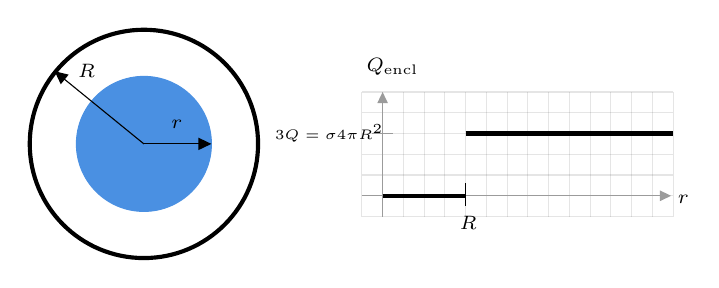
\begin{tikzpicture}[x=0.75pt,y=0.75pt,yscale=-1,xscale=1]
%uncomment if require: \path (0,128); %set diagram left start at 0, and has height of 128

%Shape: Circle [id:dp48987257334075207] 
\draw  [color={rgb, 255:red, 74; green, 144; blue, 226 }  ,draw opacity=1 ][fill={rgb, 255:red, 74; green, 144; blue, 226 }  ,fill opacity=1 ] (32.49,65) .. controls (32.49,47.04) and (47.04,32.49) .. (65,32.49) .. controls (82.96,32.49) and (97.51,47.04) .. (97.51,65) .. controls (97.51,82.96) and (82.96,97.51) .. (65,97.51) .. controls (47.04,97.51) and (32.49,82.96) .. (32.49,65) -- cycle ;
%Shape: Circle [id:dp6052140120773126] 
\draw  [line width=1.5]  (10,65) .. controls (10,34.62) and (34.62,10) .. (65,10) .. controls (95.38,10) and (120,34.62) .. (120,65) .. controls (120,95.38) and (95.38,120) .. (65,120) .. controls (34.62,120) and (10,95.38) .. (10,65) -- cycle ;
%Straight Lines [id:da3700667290172912] 
\draw    (65,65) -- (94.51,65) ;
\draw [shift={(97.51,65)}, rotate = 180] [fill={rgb, 255:red, 0; green, 0; blue, 0 }  ][line width=0.08]  [draw opacity=0] (6.25,-3) -- (0,0) -- (6.25,3) -- cycle    ;
%Straight Lines [id:da8052508879762954] 
\draw    (65,65) -- (24.33,31.89) ;
\draw [shift={(22,30)}, rotate = 39.14] [fill={rgb, 255:red, 0; green, 0; blue, 0 }  ][line width=0.08]  [draw opacity=0] (6.25,-3) -- (0,0) -- (6.25,3) -- cycle    ;
%Shape: Grid [id:dp11369043107613086] 
\draw  [draw opacity=0] (170,40) -- (320,40) -- (320,100) -- (170,100) -- cycle ; \draw  [color={rgb, 255:red, 0; green, 0; blue, 0 }  ,draw opacity=0.1 ] (170,40) -- (170,100)(180,40) -- (180,100)(190,40) -- (190,100)(200,40) -- (200,100)(210,40) -- (210,100)(220,40) -- (220,100)(230,40) -- (230,100)(240,40) -- (240,100)(250,40) -- (250,100)(260,40) -- (260,100)(270,40) -- (270,100)(280,40) -- (280,100)(290,40) -- (290,100)(300,40) -- (300,100)(310,40) -- (310,100) ; \draw  [color={rgb, 255:red, 0; green, 0; blue, 0 }  ,draw opacity=0.1 ] (170,40) -- (320,40)(170,50) -- (320,50)(170,60) -- (320,60)(170,70) -- (320,70)(170,80) -- (320,80)(170,90) -- (320,90) ; \draw  [color={rgb, 255:red, 0; green, 0; blue, 0 }  ,draw opacity=0.1 ]  ;
%Straight Lines [id:da9234529016787134] 
\draw [color={rgb, 255:red, 0; green, 0; blue, 0 }  ,draw opacity=0.1 ]   (170,100) -- (320,100) ;
%Straight Lines [id:da02274810740903832] 
\draw [color={rgb, 255:red, 0; green, 0; blue, 0 }  ,draw opacity=0.1 ]   (320,100) -- (320,40) ;

%Straight Lines [id:da5709555724750504] 
\draw [color={rgb, 255:red, 155; green, 155; blue, 155 }  ,draw opacity=1 ]   (180,43) -- (180,100) ;
\draw [shift={(180,40)}, rotate = 90] [fill={rgb, 255:red, 155; green, 155; blue, 155 }  ,fill opacity=1 ][line width=0.08]  [draw opacity=0] (5.36,-2.57) -- (0,0) -- (5.36,2.57) -- cycle    ;
%Straight Lines [id:da2981521914099221] 
\draw [color={rgb, 255:red, 155; green, 155; blue, 155 }  ,draw opacity=1 ]   (170,90) -- (316,90) ;
\draw [shift={(319,90)}, rotate = 180] [fill={rgb, 255:red, 155; green, 155; blue, 155 }  ,fill opacity=1 ][line width=0.08]  [draw opacity=0] (5.36,-2.57) -- (0,0) -- (5.36,2.57) -- cycle    ;
%Straight Lines [id:da12077626612661096] 
\draw    (220,84) -- (220,95) ;
%Straight Lines [id:da7611114679170365] 
\draw [line width=1.5]    (180,90) -- (220,90) ;
%Straight Lines [id:da004562646293197803] 
\draw [line width=1.5]    (220,60) -- (320,60) ;
%Straight Lines [id:da9946915067147775] 
\draw [color={rgb, 255:red, 155; green, 155; blue, 155 }  ,draw opacity=1 ]   (175,60) -- (185,60) ;

% Text Node
\draw (32,25.4) node [anchor=north west][inner sep=0.75pt]  [font=\scriptsize]  {$R$};
% Text Node
\draw (77,52.4) node [anchor=north west][inner sep=0.75pt]  [font=\scriptsize]  {$r$};
% Text Node
\draw (171,22.4) node [anchor=north west][inner sep=0.75pt]  [font=\scriptsize]  {$Q_{\mathrm{encl}}$};
% Text Node
\draw (216,98.4) node [anchor=north west][inner sep=0.75pt]  [font=\scriptsize]  {$R$};
% Text Node
\draw (321,88.4) node [anchor=north west][inner sep=0.75pt]  [font=\scriptsize]  {$r$};
% Text Node
\draw (127,54.4) node [anchor=north west][inner sep=0.75pt]  [font=\tiny]  {$3Q=\sigma 4\pi R^{2}$};


\end{tikzpicture}


It was found that when the radius $r$ of the Gaussian sphere is less than $R$, $Q_{\text{encl}}=0$. When the $r>R$, $Q_{\text{encl}}=+3Q$:

$$
   Q_{\text{encl}} = \begin{cases}
     0   &\text{if } r < R \\
     +3Q &\text{if } r > R
   \end{cases}
   $$

\begin{enumerate}

  \item Why can we assume that if there is an electric field, it must be radial so that the electric field will always be perpendicular to the Gaussian surface?

  \item Find $E(r)$

  \item Plot $E(r)$

\end{enumerate}

\newpage

\textbf{Answer}



\tikzset{every picture/.style={line width=0.75pt}} %set default line width to 0.75pt        

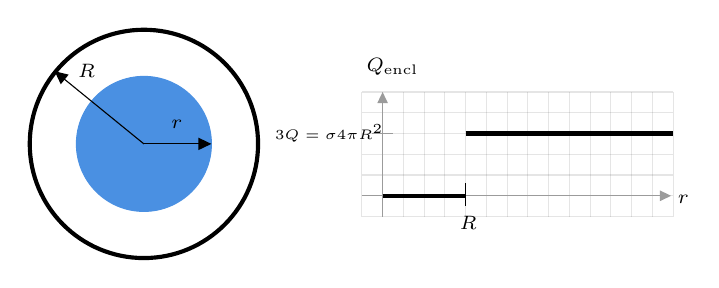
\begin{tikzpicture}[x=0.75pt,y=0.75pt,yscale=-1,xscale=1]
%uncomment if require: \path (0,128); %set diagram left start at 0, and has height of 128

%Shape: Circle [id:dp48987257334075207] 
\draw  [color={rgb, 255:red, 74; green, 144; blue, 226 }  ,draw opacity=1 ][fill={rgb, 255:red, 74; green, 144; blue, 226 }  ,fill opacity=1 ] (32.49,65) .. controls (32.49,47.04) and (47.04,32.49) .. (65,32.49) .. controls (82.96,32.49) and (97.51,47.04) .. (97.51,65) .. controls (97.51,82.96) and (82.96,97.51) .. (65,97.51) .. controls (47.04,97.51) and (32.49,82.96) .. (32.49,65) -- cycle ;
%Shape: Circle [id:dp6052140120773126] 
\draw  [line width=1.5]  (10,65) .. controls (10,34.62) and (34.62,10) .. (65,10) .. controls (95.38,10) and (120,34.62) .. (120,65) .. controls (120,95.38) and (95.38,120) .. (65,120) .. controls (34.62,120) and (10,95.38) .. (10,65) -- cycle ;
%Straight Lines [id:da3700667290172912] 
\draw    (65,65) -- (94.51,65) ;
\draw [shift={(97.51,65)}, rotate = 180] [fill={rgb, 255:red, 0; green, 0; blue, 0 }  ][line width=0.08]  [draw opacity=0] (6.25,-3) -- (0,0) -- (6.25,3) -- cycle    ;
%Straight Lines [id:da8052508879762954] 
\draw    (65,65) -- (24.33,31.89) ;
\draw [shift={(22,30)}, rotate = 39.14] [fill={rgb, 255:red, 0; green, 0; blue, 0 }  ][line width=0.08]  [draw opacity=0] (6.25,-3) -- (0,0) -- (6.25,3) -- cycle    ;
%Shape: Grid [id:dp11369043107613086] 
\draw  [draw opacity=0] (170,40) -- (320,40) -- (320,100) -- (170,100) -- cycle ; \draw  [color={rgb, 255:red, 0; green, 0; blue, 0 }  ,draw opacity=0.1 ] (170,40) -- (170,100)(180,40) -- (180,100)(190,40) -- (190,100)(200,40) -- (200,100)(210,40) -- (210,100)(220,40) -- (220,100)(230,40) -- (230,100)(240,40) -- (240,100)(250,40) -- (250,100)(260,40) -- (260,100)(270,40) -- (270,100)(280,40) -- (280,100)(290,40) -- (290,100)(300,40) -- (300,100)(310,40) -- (310,100) ; \draw  [color={rgb, 255:red, 0; green, 0; blue, 0 }  ,draw opacity=0.1 ] (170,40) -- (320,40)(170,50) -- (320,50)(170,60) -- (320,60)(170,70) -- (320,70)(170,80) -- (320,80)(170,90) -- (320,90) ; \draw  [color={rgb, 255:red, 0; green, 0; blue, 0 }  ,draw opacity=0.1 ]  ;
%Straight Lines [id:da9234529016787134] 
\draw [color={rgb, 255:red, 0; green, 0; blue, 0 }  ,draw opacity=0.1 ]   (170,100) -- (320,100) ;
%Straight Lines [id:da02274810740903832] 
\draw [color={rgb, 255:red, 0; green, 0; blue, 0 }  ,draw opacity=0.1 ]   (320,100) -- (320,40) ;

%Straight Lines [id:da5709555724750504] 
\draw [color={rgb, 255:red, 155; green, 155; blue, 155 }  ,draw opacity=1 ]   (180,43) -- (180,100) ;
\draw [shift={(180,40)}, rotate = 90] [fill={rgb, 255:red, 155; green, 155; blue, 155 }  ,fill opacity=1 ][line width=0.08]  [draw opacity=0] (5.36,-2.57) -- (0,0) -- (5.36,2.57) -- cycle    ;
%Straight Lines [id:da2981521914099221] 
\draw [color={rgb, 255:red, 155; green, 155; blue, 155 }  ,draw opacity=1 ]   (170,90) -- (316,90) ;
\draw [shift={(319,90)}, rotate = 180] [fill={rgb, 255:red, 155; green, 155; blue, 155 }  ,fill opacity=1 ][line width=0.08]  [draw opacity=0] (5.36,-2.57) -- (0,0) -- (5.36,2.57) -- cycle    ;
%Straight Lines [id:da12077626612661096] 
\draw    (220,84) -- (220,95) ;
%Straight Lines [id:da7611114679170365] 
\draw [line width=1.5]    (180,90) -- (220,90) ;
%Straight Lines [id:da004562646293197803] 
\draw [line width=1.5]    (220,60) -- (320,60) ;
%Straight Lines [id:da9946915067147775] 
\draw [color={rgb, 255:red, 155; green, 155; blue, 155 }  ,draw opacity=1 ]   (175,60) -- (185,60) ;

% Text Node
\draw (32,25.4) node [anchor=north west][inner sep=0.75pt]  [font=\scriptsize]  {$R$};
% Text Node
\draw (77,52.4) node [anchor=north west][inner sep=0.75pt]  [font=\scriptsize]  {$r$};
% Text Node
\draw (171,22.4) node [anchor=north west][inner sep=0.75pt]  [font=\scriptsize]  {$Q_{\mathrm{encl}}$};
% Text Node
\draw (216,98.4) node [anchor=north west][inner sep=0.75pt]  [font=\scriptsize]  {$R$};
% Text Node
\draw (321,88.4) node [anchor=north west][inner sep=0.75pt]  [font=\scriptsize]  {$r$};
% Text Node
\draw (127,54.4) node [anchor=north west][inner sep=0.75pt]  [font=\tiny]  {$3Q=\sigma 4\pi R^{2}$};


\end{tikzpicture}


\begin{enumerate}

  \item Pick a point in space at an arbitrary location to find the electric field. For any point, one can always find two charges on the shell whose electric field's sum is radial. Given that one can construct a uniformly charged shell by placing such pairs of points on a shell, the net electric field due to all charges on the shell must be radial. \emph{Draw a diagram to demonstrate this}.

  \item Because of our answer to 1., we can use

        $$EA = E 4\pi r^2 = \frac{Q_{\text{encl}}}{\epsilon_o}$$

        $Q_{\text{encl}}$ depends on $r$, so our answer for $E$ must also depend on $r$:

        $$
        E = \begin{cases}
          0   &\text{if } r < R \\\\
          \ds\frac{1}{4\pi\epsilon_o}\frac{3Q}{r^2} &\text{if } r > R
        \end{cases}
        $$

  \item The plot is shown below. Notice that inside the uniformly charged shell, the electric field is zero. Outside, the electric field is the same as if all of the charge ($3Q$) was at the origin. This is a result that is often used when solving other problems. You may recall from mechanics that a similar result held -- Newton showed that if the mass was uniformly distributed on a spherical shell, the gravitational force on an object inside the shell was zero; outside the shell, the gravitational force was the same as if all of the mass was at the center of the shell.

        

\tikzset{every picture/.style={line width=0.75pt}} %set default line width to 0.75pt        

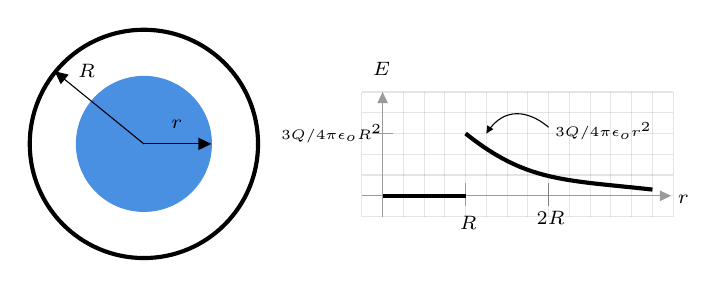
\begin{tikzpicture}[x=0.75pt,y=0.75pt,yscale=-1,xscale=1]
%uncomment if require: \path (0,128); %set diagram left start at 0, and has height of 128

%Shape: Circle [id:dp20040224525381878] 
\draw  [color={rgb, 255:red, 74; green, 144; blue, 226 }  ,draw opacity=1 ][fill={rgb, 255:red, 74; green, 144; blue, 226 }  ,fill opacity=1 ] (32.49,65) .. controls (32.49,47.04) and (47.04,32.49) .. (65,32.49) .. controls (82.96,32.49) and (97.51,47.04) .. (97.51,65) .. controls (97.51,82.96) and (82.96,97.51) .. (65,97.51) .. controls (47.04,97.51) and (32.49,82.96) .. (32.49,65) -- cycle ;
%Shape: Circle [id:dp8916595576059034] 
\draw  [line width=1.5]  (10,65) .. controls (10,34.62) and (34.62,10) .. (65,10) .. controls (95.38,10) and (120,34.62) .. (120,65) .. controls (120,95.38) and (95.38,120) .. (65,120) .. controls (34.62,120) and (10,95.38) .. (10,65) -- cycle ;
%Straight Lines [id:da7513452876992421] 
\draw    (65,65) -- (94.51,65) ;
\draw [shift={(97.51,65)}, rotate = 180] [fill={rgb, 255:red, 0; green, 0; blue, 0 }  ][line width=0.08]  [draw opacity=0] (6.25,-3) -- (0,0) -- (6.25,3) -- cycle    ;
%Straight Lines [id:da8578868115778884] 
\draw    (65,65) -- (24.33,31.89) ;
\draw [shift={(22,30)}, rotate = 39.14] [fill={rgb, 255:red, 0; green, 0; blue, 0 }  ][line width=0.08]  [draw opacity=0] (6.25,-3) -- (0,0) -- (6.25,3) -- cycle    ;
%Shape: Grid [id:dp7809548371956838] 
\draw  [draw opacity=0] (170,40) -- (320,40) -- (320,100) -- (170,100) -- cycle ; \draw  [color={rgb, 255:red, 0; green, 0; blue, 0 }  ,draw opacity=0.1 ] (170,40) -- (170,100)(180,40) -- (180,100)(190,40) -- (190,100)(200,40) -- (200,100)(210,40) -- (210,100)(220,40) -- (220,100)(230,40) -- (230,100)(240,40) -- (240,100)(250,40) -- (250,100)(260,40) -- (260,100)(270,40) -- (270,100)(280,40) -- (280,100)(290,40) -- (290,100)(300,40) -- (300,100)(310,40) -- (310,100) ; \draw  [color={rgb, 255:red, 0; green, 0; blue, 0 }  ,draw opacity=0.1 ] (170,40) -- (320,40)(170,50) -- (320,50)(170,60) -- (320,60)(170,70) -- (320,70)(170,80) -- (320,80)(170,90) -- (320,90) ; \draw  [color={rgb, 255:red, 0; green, 0; blue, 0 }  ,draw opacity=0.1 ]  ;
%Straight Lines [id:da5002568537509797] 
\draw [color={rgb, 255:red, 0; green, 0; blue, 0 }  ,draw opacity=0.1 ]   (170,100) -- (320,100) ;
%Straight Lines [id:da09134212910137607] 
\draw [color={rgb, 255:red, 0; green, 0; blue, 0 }  ,draw opacity=0.1 ]   (320,100) -- (320,40) ;

%Straight Lines [id:da31101177303364036] 
\draw [color={rgb, 255:red, 155; green, 155; blue, 155 }  ,draw opacity=1 ]   (180,43) -- (180,100) ;
\draw [shift={(180,40)}, rotate = 90] [fill={rgb, 255:red, 155; green, 155; blue, 155 }  ,fill opacity=1 ][line width=0.08]  [draw opacity=0] (5.36,-2.57) -- (0,0) -- (5.36,2.57) -- cycle    ;
%Straight Lines [id:da17469793011953216] 
\draw [color={rgb, 255:red, 155; green, 155; blue, 155 }  ,draw opacity=1 ]   (170,90) -- (316,90) ;
\draw [shift={(319,90)}, rotate = 180] [fill={rgb, 255:red, 155; green, 155; blue, 155 }  ,fill opacity=1 ][line width=0.08]  [draw opacity=0] (5.36,-2.57) -- (0,0) -- (5.36,2.57) -- cycle    ;
%Straight Lines [id:da059953978515083106] 
\draw [color={rgb, 255:red, 155; green, 155; blue, 155 }  ,draw opacity=1 ]   (220,84) -- (220,95) ;
%Straight Lines [id:da24478782587243564] 
\draw [line width=1.5]    (180,90) -- (220,90) ;
%Straight Lines [id:da27346654142823046] 
\draw [color={rgb, 255:red, 155; green, 155; blue, 155 }  ,draw opacity=1 ]   (175,60) -- (185,60) ;
%Curve Lines [id:da46273645063648505] 
\draw [line width=1.5]    (220,60) .. controls (249.2,83.28) and (267.2,82.28) .. (310,87) ;
%Curve Lines [id:da7493706286742585] 
\draw    (231.84,57.37) .. controls (240.87,45.94) and (252.71,50.72) .. (260,57) ;
\draw [shift={(230,60)}, rotate = 302.01] [fill={rgb, 255:red, 0; green, 0; blue, 0 }  ][line width=0.08]  [draw opacity=0] (3.57,-1.72) -- (0,0) -- (3.57,1.72) -- cycle    ;
%Straight Lines [id:da7285565346879526] 
\draw [color={rgb, 255:red, 128; green, 128; blue, 128 }  ,draw opacity=1 ]   (260,84) -- (260,95) ;

% Text Node
\draw (32,25.4) node [anchor=north west][inner sep=0.75pt]  [font=\scriptsize]  {$R$};
% Text Node
\draw (77,52.4) node [anchor=north west][inner sep=0.75pt]  [font=\scriptsize]  {$r$};
% Text Node
\draw (174,24.4) node [anchor=north west][inner sep=0.75pt]  [font=\scriptsize]  {$E$};
% Text Node
\draw (216,98.4) node [anchor=north west][inner sep=0.75pt]  [font=\scriptsize]  {$R$};
% Text Node
\draw (321,88.4) node [anchor=north west][inner sep=0.75pt]  [font=\scriptsize]  {$r$};
% Text Node
\draw (130,54.4) node [anchor=north west][inner sep=0.75pt]  [font=\tiny]  {$3Q/4\pi \epsilon _{o} R^{2}$};
% Text Node
\draw (262,53.4) node [anchor=north west][inner sep=0.75pt]  [font=\tiny]  {$3Q/4\pi \epsilon _{o} r^{2}$};
% Text Node
\draw (253,96.37) node [anchor=north west][inner sep=0.75pt]  [font=\scriptsize]  {$2R$};


\end{tikzpicture}


\end{enumerate}

\newpage

\section{Problem -- Solid Sphere With Uniform Charge Density}

In the Enclosed Charge activity, a non--conducting sphere of radius $R$ has a charge of $+3Q$ distributed uniformly \emph{throughout} it was considered. The cross--section of the sphere is shown along with a dashed line representing the surface of a Gaussian sphere, which has the same center as the charged sphere and a radius $r$.



\tikzset{every picture/.style={line width=0.75pt}} %set default line width to 0.75pt        

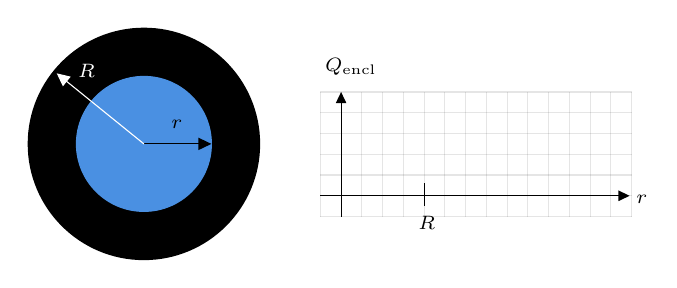
\begin{tikzpicture}[x=0.75pt,y=0.75pt,yscale=-1,xscale=1]
%uncomment if require: \path (0,128); %set diagram left start at 0, and has height of 128

%Shape: Circle [id:dp9766835204632047] 
\draw  [fill={rgb, 255:red, 0; green, 0; blue, 0 }  ,fill opacity=1 ][line width=1.5]  (10,65) .. controls (10,34.62) and (34.62,10) .. (65,10) .. controls (95.38,10) and (120,34.62) .. (120,65) .. controls (120,95.38) and (95.38,120) .. (65,120) .. controls (34.62,120) and (10,95.38) .. (10,65) -- cycle ;
%Shape: Circle [id:dp5025968278267186] 
\draw  [color={rgb, 255:red, 74; green, 144; blue, 226 }  ,draw opacity=1 ][fill={rgb, 255:red, 74; green, 144; blue, 226 }  ,fill opacity=1 ] (32.49,65) .. controls (32.49,47.04) and (47.04,32.49) .. (65,32.49) .. controls (82.96,32.49) and (97.51,47.04) .. (97.51,65) .. controls (97.51,82.96) and (82.96,97.51) .. (65,97.51) .. controls (47.04,97.51) and (32.49,82.96) .. (32.49,65) -- cycle ;
%Straight Lines [id:da579089752665406] 
\draw    (65,65) -- (94.51,65) ;
\draw [shift={(97.51,65)}, rotate = 180] [fill={rgb, 255:red, 0; green, 0; blue, 0 }  ][line width=0.08]  [draw opacity=0] (6.25,-3) -- (0,0) -- (6.25,3) -- cycle    ;
%Straight Lines [id:da3113687194658947] 
\draw [color={rgb, 255:red, 255; green, 255; blue, 255 }  ,draw opacity=1 ]   (65,65) -- (25.33,32.89) ;
\draw [shift={(23,31)}, rotate = 38.99] [fill={rgb, 255:red, 255; green, 255; blue, 255 }  ,fill opacity=1 ][line width=0.08]  [draw opacity=0] (6.25,-3) -- (0,0) -- (6.25,3) -- cycle    ;
%Shape: Grid [id:dp4072097255438287] 
\draw  [draw opacity=0] (150,40) -- (300,40) -- (300,100) -- (150,100) -- cycle ; \draw  [color={rgb, 255:red, 0; green, 0; blue, 0 }  ,draw opacity=0.1 ] (150,40) -- (150,100)(160,40) -- (160,100)(170,40) -- (170,100)(180,40) -- (180,100)(190,40) -- (190,100)(200,40) -- (200,100)(210,40) -- (210,100)(220,40) -- (220,100)(230,40) -- (230,100)(240,40) -- (240,100)(250,40) -- (250,100)(260,40) -- (260,100)(270,40) -- (270,100)(280,40) -- (280,100)(290,40) -- (290,100) ; \draw  [color={rgb, 255:red, 0; green, 0; blue, 0 }  ,draw opacity=0.1 ] (150,40) -- (300,40)(150,50) -- (300,50)(150,60) -- (300,60)(150,70) -- (300,70)(150,80) -- (300,80)(150,90) -- (300,90) ; \draw  [color={rgb, 255:red, 0; green, 0; blue, 0 }  ,draw opacity=0.1 ]  ;
%Straight Lines [id:da5916223647803596] 
\draw [color={rgb, 255:red, 0; green, 0; blue, 0 }  ,draw opacity=0.1 ]   (150,100) -- (300,100) ;
%Straight Lines [id:da028168436365389127] 
\draw [color={rgb, 255:red, 0; green, 0; blue, 0 }  ,draw opacity=0.1 ]   (300,100) -- (300,40) ;

%Straight Lines [id:da0004616455927557439] 
\draw    (160,43) -- (160,100) ;
\draw [shift={(160,40)}, rotate = 90] [fill={rgb, 255:red, 0; green, 0; blue, 0 }  ][line width=0.08]  [draw opacity=0] (5.36,-2.57) -- (0,0) -- (5.36,2.57) -- cycle    ;
%Straight Lines [id:da7260057623276042] 
\draw [color={rgb, 255:red, 0; green, 0; blue, 0 }  ,draw opacity=1 ]   (150,90) -- (296,90) ;
\draw [shift={(299,90)}, rotate = 180] [fill={rgb, 255:red, 0; green, 0; blue, 0 }  ,fill opacity=1 ][line width=0.08]  [draw opacity=0] (5.36,-2.57) -- (0,0) -- (5.36,2.57) -- cycle    ;
%Straight Lines [id:da5178691434385663] 
\draw    (200,84) -- (200,95) ;

% Text Node
\draw (32,25.4) node [anchor=north west][inner sep=0.75pt]  [font=\scriptsize,color={rgb, 255:red, 255; green, 255; blue, 255 }  ,opacity=1 ]  {$R$};
% Text Node
\draw (77,52.4) node [anchor=north west][inner sep=0.75pt]  [font=\scriptsize]  {$r$};
% Text Node
\draw (151,22.4) node [anchor=north west][inner sep=0.75pt]  [font=\scriptsize]  {$Q_{\mathrm{encl}}$};
% Text Node
\draw (196,98.4) node [anchor=north west][inner sep=0.75pt]  [font=\scriptsize]  {$R$};
% Text Node
\draw (301,88.4) node [anchor=north west][inner sep=0.75pt]  [font=\scriptsize]  {$r$};


\end{tikzpicture}


$$
Q_{\text{encl}} = \begin{cases}
  \rho_o [(4/3)\pi r^3]   &\text{if  }r \le R \\\\
  \rho_o [(4/3)\pi R^3] &\text{if } r \ge R
\end{cases}
$$

where $\ds \rho_o=3Q/[(4/3)\pi R^3]$

\begin{enumerate}

  \item Why can we assume that if there is an electric field, it must be radial so that the electric field will always be perpendicular to the Gaussian surface?

        \ifsolutions

        \else
        \vskip 96pt
        \fi

  \item Find $E(r)$

        \ifsolutions

        \else
        \vskip 96pt
        \fi

  \item Plot $E(r)$

        \ifsolutions

        \else
        \vskip 96pt
        \fi

\end{enumerate}

\newpage

\section{Problem -- Solid Sphere With Non--Uniform Charge Density}

Suppose the charged sphere in the previous problem had a charge density that varied with radius according to $\rho(r) = \rho_o r/R$.

\begin{enumerate}

  \item Why can we assume that if there is an electric field, it must be radial so that the electric field will always be perpendicular to the Gaussian surface?

        \ifsolutions

        \else
        \vskip 96pt
        \fi

  \item Find $Q_{\text{encl}}(r)$

        \ifsolutions

        \else
        \vskip 144pt
        \fi

  \item Find $E(r)$

        \ifsolutions

        \else
        \vskip 144pt
        \fi

  \item Plot $E(r)$

\end{enumerate}

\end{document}